\phantomsection
\subsubsection*{Դասերի համար հարցումներ}\label{subsubsec:classes}
\addcontentsline{toc}{subsubsection}{Դասերի համար հարցումներ}

Այս հարցումները բաժանվում են երկու խմբի՝
\begin{enumerate}
    \item որոնման հարցումներ,
    \item դասի վերլուծության հարցումներ:
\end{enumerate}

Որոնման հարցումների միջոցով օգտագործողները կարող են որոնել և գտնել ծրագրի դասերն՝ օգտագործելով տարբեր ֆիլտրեր:
Նրանք կարող են որոնել դասերն ըստ՝
\begin{enumerate}
    \item անվանման,
    \item պարունակող կամ չպարունակող ֆունկցիաների,
    \item անդամ դաշտերի և այլն։
\end{enumerate}

Սա թույլ կտա օգտագործողներին արագ և թիրախավորված կերպով գտնել իրենց հետաքրքրող դասերը:

Երբ օգտագործողը ընտրել է կոնկրետ դաս, նա կարող է անցնել դրա մանրամասն վերլուծությանը: Այդ դասի վերլուծության
հարցումների միջոցով հնարավոր կլինի ստանալ տեղեկություններ՝
\begin{enumerate}
    \item դասի ծնող և ժառանգ դասերի մասին,
    \item անդամ ֆունկցիաների մասին,
    \item անդամ դաշտերի մասին և այլն։
\end{enumerate}

Նկար \ref{fig:figure13}-ում դասերի հարցումների օրինակ է։ Այս օրինակում օգտագործողը որոնման հարցումների միջոցով գտնուն է
"\_class" անվանման վերջավորություն ունեցող դասերը (class1), այնուհետև գտնում է "d" անունով ֆունկցիա պարունակող դասերը (class2)
և գտնում է այդ երկու բազմությունների տարբերությունը (diff1)։ Այս ամենը կատարվում է տվյալների բազային մեկ անգամ դիմելով (exec())։

\begin{figure}[h]
    \centering
    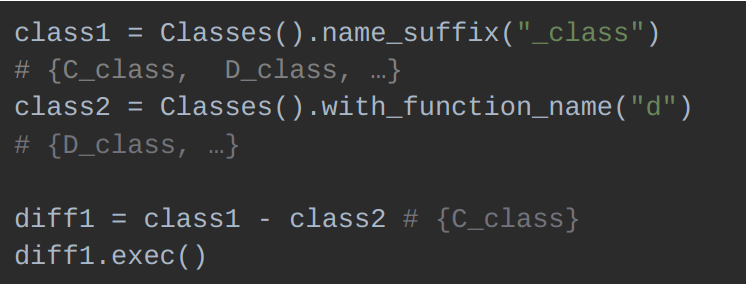
\includegraphics[width=0.6\textwidth]{pic13}
    \caption{Դասերի համար հարցումների օրինակ}
    \label{fig:figure13}
\end{figure}

Այսպիսով, դասերի համար նախատեսված որոնման և վերլուծության հարցումները թույլ կտան օգտագործողներին տեղեկանալ դասերի
և դրանց կապերի մասին:
